\documentclass[border=10pt]{standalone}

\usepackage{tikz}
\usepackage{tikzsymbols}
\usetikzlibrary{calc,patterns,shapes.geometric}

\def\centerarc[#1](#2)(#3:#4:#5){\draw[#1] ($(#2)+({#5*cos(#3)},{#5*sin(#3)})$) arc (#3:#4:#5);}

\begin{document}
	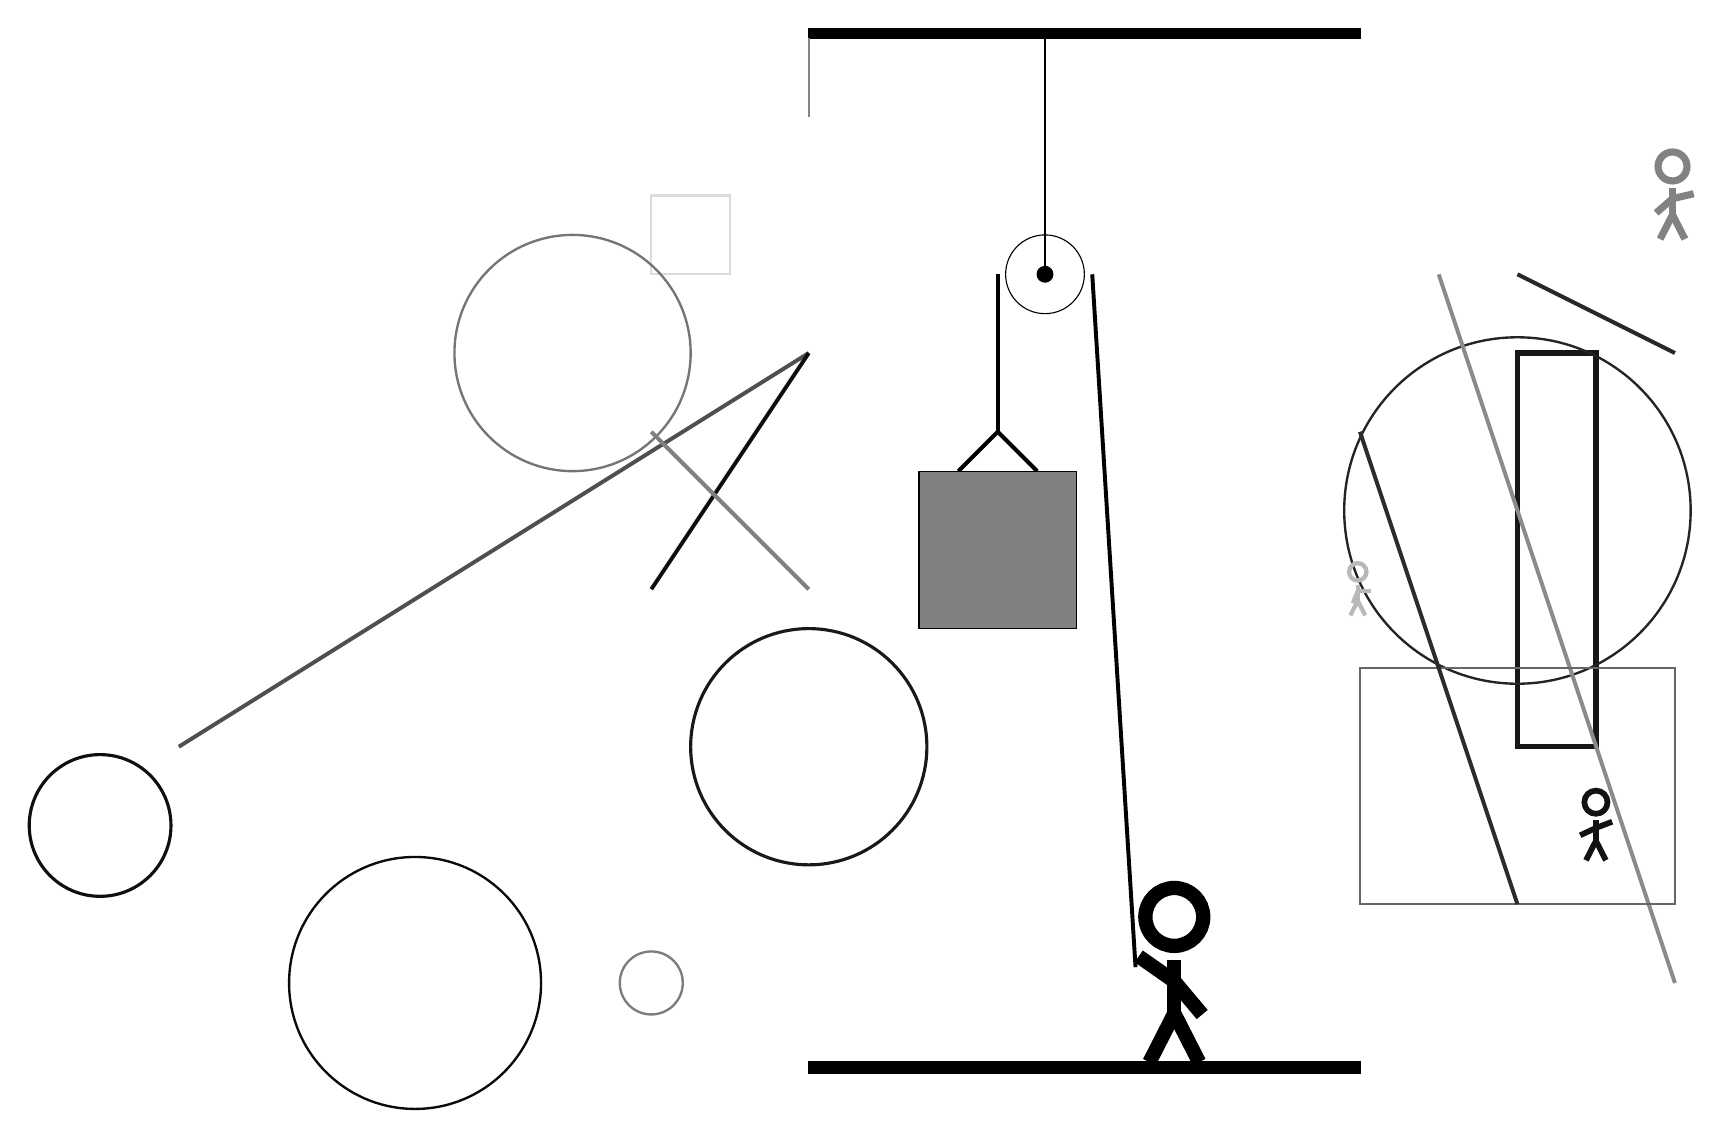
\begin{tikzpicture}
		%%%%% START %%%%%
		
		\draw[fill=black] (-2, 10) rectangle (5, 10.125);
		
		\draw (1, 7) circle (0.5);
		\draw[fill=black] (1, 7) circle (0.1);
		\draw (1, 10) -- (1, 7);
		
		\draw[line width=0.7mm, color=black!91] (7, 1) rectangle (8, 6);
		
		\node[line width=0.6mm, color=black!93] at (8, 0) {\Strichmaxerl[4][25][21]};
		\draw[line width=0.5mm, color=black!84](9, 6) -- (7, 7);
		\draw[line width=0.3mm, color=black!48] (-2, 10) rectangle (-2, 9);
		\draw [line width=0.3mm, color=black!51](-4, -2) circle (0.4);
		\draw [line width=0.3mm, color=black!86](7, 4) circle (2.2);
		
		\draw[line width=0.5mm, color=black!69](-2, 6) -- (-10, 1);
		\draw [line width=0.4mm, color=black!90](-2, 1) circle (1.5);
		\node[line width=0.4mm, color=black!49] at (9, 8) {\Strichmaxerl[5][41][13]};
		
		\draw[line width=0.5mm, color=black!46](6, 7) -- (9, -2);
		\draw [line width=0.4mm, color=black!94](-11, 0) circle (0.9);
		
		\draw[line width=0.3mm, color=black!14] (-4, 7) rectangle (-3, 8);
		\draw [line width=0.3mm, color=black!96](-7, -2) circle (1.6);
		
		\draw [line width=0.3mm, color=black!54](-5, 6) circle (1.5);
		\draw[line width=0.5mm, color=black!94](-4, 3) -- (-2, 6);
		\draw[line width=0.5mm, color=black!50](-2, 3) -- (-4, 5);
		\draw[line width=0.3mm, color=black!60] (5, 2) rectangle (9, -1);
		\draw[line width=0.5mm, color=black!83](7, -1) -- (5, 5);
		\node[line width=0.7mm, color=black!28] at (5, 3) {\Strichmaxerl[3][68][0]};
		
		\draw[line width=0.5mm] (-0.1, 4.5) -- (0.4, 5.0) -- (0.9, 4.5);
		\draw[fill=black!50] (-0.6, 4.5) rectangle (1.4, 2.5);
		
		\draw[line width=0.5mm] (0.4, 7) -- (0.4, 5.0);
		\centerarc[line width=0.5mm](1, 7)(0:180:0.6);
		\draw[line width=0.5mm](1.6, 7) -- (2.15, -1.8);
		
		\node at (2.6, -1.9) {\Strichmaxerl[10][-35][-50]};
		
		\draw[fill=black] (-2, -3) rectangle (5, -3.15);
		
		%%%%% END %%%%%
	\end{tikzpicture}
\end{document}